\documentclass[11pt,a4paper]{article}
\usepackage[margin=25mm]{geometry}
\usepackage[T1]{fontenc}
\usepackage{lmodern,microtype,graphicx,booktabs,tabularx,array,amsmath,amssymb}
\usepackage[round,authoryear]{natbib}
\usepackage[colorlinks=true,allcolors=blue!45!black]{hyperref}
\usepackage{xcolor,fancyhdr,caption,float}
\usepackage[section]{placeins}
\hypersetup{pdftitle={After Krypton: Realization, Uncertainty, and the Uneven Remaking of the Metre, 1983--2000},pdfauthor={Shivam Gupta}}
\graphicspath{{../figures/}}
\captionsetup{font=small,labelfont=bf}
\setlength{\parskip}{4pt}\setlength{\parindent}{1em}
\setlength{\emergencystretch}{2em}
\pagestyle{fancy}\fancyhf{}\fancyhead[L]{\small Gupta | After Krypton}\fancyhead[R]{\small Research manuscript}\fancyfoot[C]{\thepage}
\newcolumntype{Y}{>{\raggedright\arraybackslash}X}
\title{After Krypton:\\Realization, Uncertainty, and the Uneven\\Remaking of the Metre, 1983--2000}
\author{Shivam Gupta\\\small Independent Scholar, India\\\small\href{mailto:shivam1720406@gmail.com}{shivam1720406@gmail.com}}
\date{16 October 2026}
\begin{document}
\maketitle
\begin{abstract}
In 1983 the General Conference on Weights and Measures abolished the krypton-based definition of the metre while expressly permitting continued use of its standard radiation. What changed when a source ceased to define a unit but remained an authorized means of realizing it? This paper reconstructs the relationship between definition, recommended realization, and laboratory maintenance through international decisions, three editions of the recommended-radiation list, and Canadian calibration records. A source-linked dataset distinguishes 31 individually assigned radiation regimes from twelve inherited lamp lines. All twelve legacy wavelength values recur unchanged between the 1963 recommendation and the expanded 1997 list. Four longitudinal comparisons show why uncertainty conventions and operating conditions must be preserved: the 633 nm recommendation changes by a factor of 13.6 on the explicitly stated standard-deviation basis, rather than the factor of 40 suggested by mixing conventions. A reconstruction of a Canadian uncertainty budget locates the small contribution of laser calibration within a larger instrumental system. The argument is that redefinition reorganized the authority of existing sources through revisable, conditional recommendations. It did not synchronize their retirement. This case identifies how international standardization accommodated technical improvement and service continuity within one unit of length.
\end{abstract}
\noindent\textbf{Keywords:} history of metrology; metre; measurement uncertainty; standards; instrumentation; maintenance; computational history.

\section{The problem of an authorized survivor}
The decision of October 1983 contains an apparent tension. It abolished the definition of the metre adopted in 1960, which had privileged one transition of krypton-86. Yet the same resolution anticipated practical instructions that could retain that radiation. Abolition applied to its defining status, rather than to every permissible use of the source \citep{cgpm1983}. A chronology of successive definitions can record the first action accurately while leaving the second action analytically underdeveloped.

This paper asks how that survival was organized. What authority did an older source have after losing its defining role? How did later revisions distinguish retained apparatus from more demanding realizations? What evidence connects international recommendations to the continuing work of a calibration laboratory? These questions concern the governance and material practice of physical measurement. They are not questions about whether the speed of light changed or whether the new unit was physically discontinuous.

The central argument is that the transition redistributed authority across three layers: a stable definition, amendable recommendations for realization, and locally maintained measurement systems. Their timescales differed. A source could lose constitutional importance in the definition yet retain operational legitimacy in a recommendation. A recommendation could improve without every laboratory adopting its most demanding regime. A laboratory could replace a source to support image processing while retaining much of its measuring procedure. The surviving sources were therefore more than residual objects on a path toward extinction: their continued use was expressly accommodated, with specified uncertainties and conditions.

This is a bounded historical reconstruction. It combines decisions and technical reports with arithmetic that can be rerun from transcribed data. The calculations do not make a historical interpretation true by themselves. They establish which numerical comparisons the documents permit, expose the consequences of flattening unlike entries, and constrain claims about technical replacement. The contribution is the conjunction of that reconstruction with an account of conditional authorization and maintenance. Neither the distinction between definition and realization nor the continued presence of spectral lamps is presented as a new discovery.

\section{Historiography and the scope of the contribution}
Metrological universality has long been understood as an achievement requiring material work. \citet{oconnell1993} shows how circulating particular objects and sustaining chains of comparison make apparently universal measurements possible. That perspective makes it unhelpful to describe the fixing of a constant as the disappearance of material standards. The relevant historical question is how the relations among them changed. \citet{mitchell2017} likewise locate measurement within practices of making, modeling, and metrology, rather than treating it solely as the assignment of numbers to pre-existing quantities.

Practitioner histories already explain the physics and institutional logic of the 1983 change. \citet{jennings1987} explicitly examine continuity between measurements referred to krypton and the fixed value of the speed of light. Their report is valuable as a participant account of how the new definition was justified, not simply as a store of current numerical facts. \citet{hall2006} recalls the difficulty of choosing among competing laser systems when performance, cost, and complexity did not single out an overwhelmingly superior candidate. His retrospective discussion suggests that the appeal of fixing the speed of light included avoiding dependence on one particular proposed source. It cannot, by itself, establish the motives of every delegation.

The technical literature also makes the history of recommendations unusually visible. Quinn's international reports publish the 1992 and 1997 realizations and their supporting material \citep{quinn1994,quinn1999}. More recently, \citet{schodel2021} explain the broad range of methods encompassed by the metre's practical realization and emphasize continuity across redefinitions. The present study therefore does not claim to reveal previously unnoticed physical compatibility, invent a realization procedure, or discover that recommendations evolve.

Its narrower contribution is a longitudinal comparison in which the unit of analysis is an \emph{assigned realization regime}, rather than a spectral label alone. This reveals three changes that a list of headline uncertainties obscures: a shift in reporting convention, subdivision into modes requiring different physical conditions, and reclassification without withdrawal. The reconstruction then connects this documentary structure to a Canadian laboratory's account of staged modernization. The interpretation is historical: revisable recommendations allowed institutions to recognize both improving precision and persistent service obligations.

The literature search combined terms for the metre, krypton, \emph{mise en pratique}, 1983, 1992, 1997, uncertainty, metrology, history, and maintenance. It located the directly relevant practitioner reports and the established historiography above. The exact compilation and comparison offered here were not located in that search. This is a statement about the search, not proof of universal priority. In particular, the underlying recommendations and most individual numerical facts were already public and extensively discussed in technical literature.

\section{Sources and reproducible method}
\subsection{A deliberately bounded documentary corpus}
The core sources are the 1960 and 1983 CGPM definitions; the 1975 speed-of-light recommendation; the 1963 secondary-wavelength recommendation; and the CIPM practical-realization lists adopted in 1983, 1992, and 1997 \citep{cgpm1960,cipm1963,cgpm1975,cgpm1983,cipm1983,cipm1992,cipm1997}. Institutional decisions are evidence of authorization. They are not a census of working instruments. Two additional source types test the reach of that evidence: the BIPM's 1992 technical activity report and Canadian reports on gauge-block calibration and its modernization \citep[pp.~163--164]{cipm1992}; \citep{decker1997,decker2000}.

The dataset records each separately numbered frequency or wavelength assignment in the three practical-realization lists. It contains six entries in 1983, ten in 1992, and fifteen in 1997: 31 documentary entries overall. The two methane subentries in each later list count separately because they specify distinct regimes. The twelve inherited lamp lines are stored separately. The 1983 and 1992 lists retain these by reference to the 1963 recommendation; the 1997 list prints them explicitly. Direct transcription from the 1963 proceedings permits an exact comparison of their numerical wavelengths after unit conversion.

These counts are not totals of every permissible realization. General substitution clauses allow related components when frequency differences are sufficiently well known. Some additional transitions are given as offsets or referred to appendices. Relaxed iodine conditions also appear by reference. Counting those possibilities as if they were individually numbered assignments would create a denominator with a different meaning. Table~\ref{tab:corpus} specifies the boundary.

\begin{table}[htbp]\centering\small
\caption{Documentary enumeration. A row is an assigned regime, not an independent experiment.}\label{tab:corpus}
\begin{tabularx}{\linewidth}{lrrY}\toprule
Edition & Laser regimes & Krypton line & Treatment of other lamp lines\\\midrule
1983 & 5 & 1 & 1963 recommendation retained by reference\\
1992 & 9 & 1 & Same incorporation by reference\\
1997 & 14 & 1 & Twelve lines printed in section 2.2\\\bottomrule
\end{tabularx}
\vspace{3pt}\par\footnotesize The 1997 laser total includes the 576 nm dye or frequency-doubled He--Ne entry in section 2.3. Its placement under ``spectral lamps and other sources'' does not turn it into a lamp.
\end{table}

\subsection{Transcription, matching, and checks}
Each record preserves the source section, absorbing species, transition label, operating mode, frequency unit, vacuum wavelength, uncertainty convention, and conditions. A shared family identifier helps compare editions but does not assert apparatus equivalence. The 633 nm labels $i$ and $a_{13}$, for example, are explicit aliases in the later documents. Methane's resolved and unresolved structures remain separate. The 576 nm entry is retained in the enumeration, but no 1983--1992 uncertainty ratio is used for it here, avoiding dependence on an unverified component-label equivalence.

The data retain the stated 1983 relative standard deviations alongside overall relative uncertainties. Later standard uncertainties are stored separately from expanded uncertainties. This provides a transparent comparison on the stated standard-deviation basis; it does not retrospectively assert that all uncertainty evaluations followed an identical modern protocol. The rounded overall values are not divided by three when a more specific standard-deviation figure is printed.

Source comparison also matters at the digit level. The online English 1992 recommendation gives the unresolved methane wavelength with the unit m. The bilingual proceedings give fm at printed page 142, PDF page 160. That reading is consistent with the listed frequency and with the neighboring resolved entry. The dataset uses fm and documents the correction; it does not silently treat the HTML as flawless. The English-language URL for the 1983 recommendation currently renders French text, so its numerical assignments were checked against the proceedings and the English reproduction in \citet[pp.~13--14]{jennings1987}.

The code checks frequency--wavelength consistency using decimal arithmetic:
\begin{equation}
 \epsilon_i=\lambda_i-\frac{c}{f_i},\qquad c=299\,792\,458\ \mathrm{m\,s^{-1}}.
\end{equation}
All 28 assigned frequency--wavelength pairs agree within half the last printed wavelength unit. The three krypton entries supply wavelengths only and are excluded from that check. Twelve independently transcribed legacy wavelengths agree exactly between 1963 and 1997 after conversion from units of $10^{-10}$ m to pm. Additional tests check enumeration, convention-aware ratios, methane subdivision, the reclassified laser, and the Canadian budget arithmetic. These tests validate transcription and calculation properties; they do not independently validate the original measurements.

\section{From a privileged transition to revisable routes}
The 1960 definition gave a specific krypton-86 transition a privileged constitutive position. The 1963 recommendation already supported other krypton, mercury, and cadmium radiations for interferometric measurement. Plural instruments and secondary wavelengths thus predated 1983 \citep{cgpm1960,cipm1963}. The subsequent change cannot be described as the invention of practical plurality.

The 1975 recommendation supplied a value for the speed of electromagnetic waves in vacuum while acknowledging that the uncertainty of the metre's realization constrained the evidence \citep{cgpm1975}. The 1983 decision then fixed that value in defining the unit and explicitly sought continuity within the uncertainty of the best krypton realizations. It also recognized that the instructions for practical realization could retain the old orange radiation \citep{cgpm1983}. Definition and realization were coupled but no longer tied to a single privileged transition in the same way.

The 1983 instructions authorized three routes: propagation over a measured time, wavelength obtained from measured frequency, or specified radiations used under the recommended conditions. Corrections for actual physical circumstances remained necessary. The listed-radiation route allowed a laboratory to work with an accepted assigned wavelength rather than construct its own absolute optical-frequency measurement chain \citep{cipm1983}. The precise choice of route mattered for implementation even though each was directed toward the same unit.

Krypton illustrates the change in authority particularly clearly. Its listed wavelength was $605\,780\,210$ fm in 1983 and $605\,780\,210.3$ fm in the later lists. The numerical shift is about $4.95\times10^{-10}$ relative, smaller than the stated $1.3\times10^{-9}$ relative standard-deviation figure. This comparison establishes scale, not a significance test: the estimates are historically related, and independence is not assumed. Krypton continued as a conditional recommended source, with a nonzero assigned uncertainty, rather than retaining its former defining position.

\begin{figure}[htbp]\centering
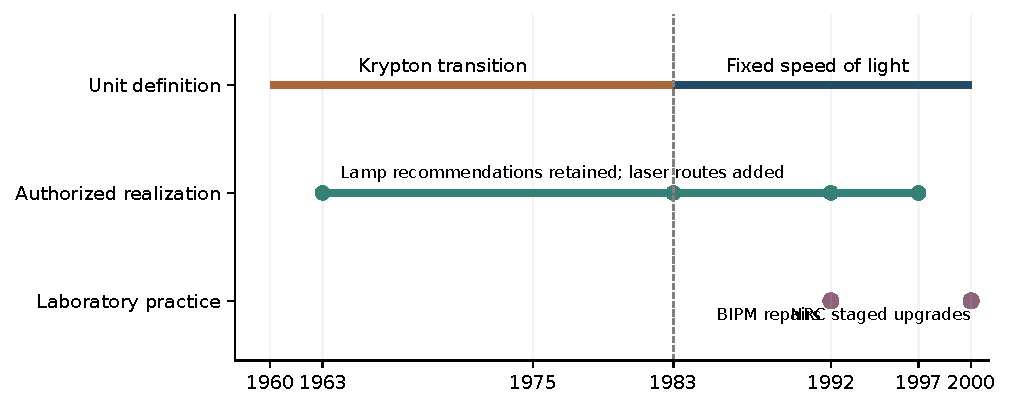
\includegraphics[width=\linewidth]{authority_layers.pdf}
\caption{Three documentary timescales. The 1983 change in definition coexisted with retained lamp recommendations and later maintenance activity. The lower markers are selected documented episodes, not observations of adoption rates. Sources: CGPM and CIPM decisions; BIPM 1992 activity report; NRC 42753.}\label{fig:layers}
\end{figure}

The older secondary wavelengths also persisted. Four krypton, four mercury, and four cadmium values in the 1963 recommendation match the twelve printed in 1997. Their retention across 34 years is an exact documentary result. It does not show that every source was still commercially available or used in every member country. It does show that international recognition did not move in lockstep with the lowest uncertainty attainable by a newer system. The register accommodated a range of capabilities within the same definition.

\section{Why the uncertainty trajectory is not one improvement curve}
\subsection{Reporting convention changes the apparent size of progress}
A comparison of numbers without their conventions creates an avoidable historical error. For the 633 nm iodine-stabilized He--Ne recommendation, 1983 gives an overall relative uncertainty of $10^{-9}$ and an estimated relative standard deviation of $3.4\times10^{-10}$. The later recommendation gives a relative standard uncertainty of $2.5\times10^{-11}$. Dividing the first overall value by the later standard uncertainty produces 40. Comparing the explicitly stated standard-deviation quantities instead produces 13.6. Both calculations are arithmetically straightforward; only the latter preserves the stated statistical scale.

Table~\ref{tab:ratios} extends the comparison to four identified families. The differences are not a uniform factor of exactly three because the original reported quantities are rounded. For methane's cell regime, the respective ratios are approximately 5.65 and 1.91. The 612 nm recommendation changes from a standard-deviation figure of $3.7\times10^{-10}$ to $3.0\times10^{-10}$, a much more modest numerical change than the 633 nm case.

\begin{table}[htbp]\centering\small
\caption{1983--1992 ratios of assigned uncertainties. ``Mixed'' divides the 1983 overall figure by the 1992 standard uncertainty and is shown only to diagnose an invalid comparison.}\label{tab:ratios}
\begin{tabular}{lrrrr}\toprule
Family & 1983 standard* & 1992 standard & Matched scale & Mixed\\\midrule
Methane cell & $4.4\times10^{-11}$ & $2.3\times10^{-11}$ & 1.91 & 5.65\\
Iodine 633 nm & $3.4\times10^{-10}$ & $2.5\times10^{-11}$ & 13.60 & 40.00\\
Iodine 612 nm & $3.7\times10^{-10}$ & $3.0\times10^{-10}$ & 1.23 & 3.67\\
Iodine 515 nm & $4.3\times10^{-10}$ & $2.5\times10^{-10}$ & 1.72 & 5.20\\\bottomrule
\end{tabular}
\par\footnotesize *Estimated relative standard deviation as printed in 1983. Ratios describe documentary assignments, not a controlled comparison of unchanged instruments. Sources: CIPM 1983, section 1; CIPM 1992, section 1.
\end{table}

\subsection{Operating conditions are part of the assigned result}
Even a convention-aware ratio does not identify an improvement of the same apparatus under identical conditions. The 633 nm recommendation tightened several operating ranges. The cell-wall range changed from $16$--$50\,^{\circ}\mathrm C$ to $25\pm5\,^{\circ}\mathrm C$. The cold-finger tolerance narrowed from $\pm1\,^{\circ}\mathrm C$ to $\pm0.2\,^{\circ}\mathrm C$, and the peak-to-peak modulation tolerance from $\pm1$ MHz to $\pm0.3$ MHz. The later entry also limits the power-shift coefficient \citep{cipm1983,cipm1992}.

\begin{figure}[htbp]\centering
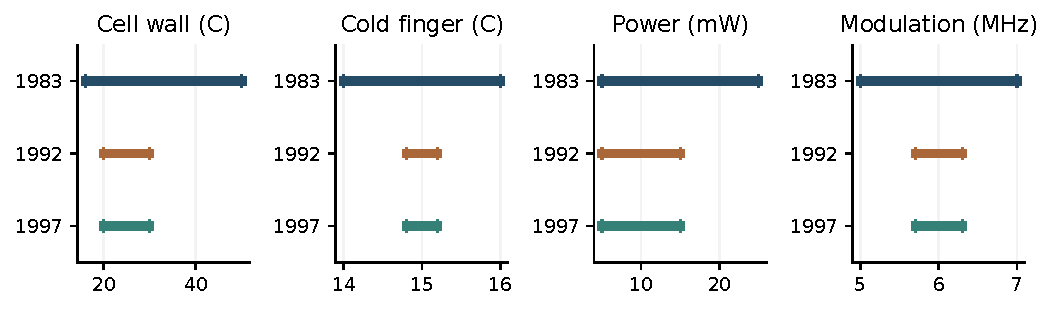
\includegraphics[width=\linewidth]{iodine_conditions.pdf}
\caption{Specified ranges for the 633 nm iodine regime. Ranges represent permitted operating conditions, not measurement-error bars. The unchanged intervals between 1992 and 1997 coexist with additional technical wording and continuing good-practice requirements. The graphic omits non-interval requirements such as the power-shift coefficient.}\label{fig:conditions}
\end{figure}

The 1992 recommendation explicitly warns that satisfying the named parameters alone is insufficient. Optical and electronic control systems must perform appropriately, and a relaxed regime carries a different uncertainty. The 1997 entry additionally names third-harmonic detection \citep{cipm1992,cipm1997}. A historian who extracts only the lowest uncertainty erases the conditions and expertise that make that number authoritative. The documents themselves preserve a boundary between following a parameter list and achieving a realization.

\subsection{A spectral family can contain different regimes}
Methane demonstrates a second problem with a single improvement curve. In 1992 the familiar room-temperature cell regime coexists with a resolved hyperfine regime that uses the central component, recoil averaging, and corrections for effectively stationary molecules. Their assigned standard uncertainties are $2.3\times10^{-11}$ and $3\times10^{-12}$ respectively. The ratio between the 1983 cell figure and the latter is 14.67, while the closer cell-to-cell comparison is 1.91. Selecting the later minimum changes the question from what happened to a retained regime to what a more demanding regime could achieve.

Calcium makes the distinction more pronounced. The 1992 recommendation specifies a thermal atomic beam and $4.5\times10^{-10}$ relative standard uncertainty. The 1997 recommendation specifies effectively stationary atoms, the mean of recoil-split components, and second-order Doppler correction, with $6\times10^{-13}$ assigned uncertainty. The numerical ratio is 750. It is not a 750-fold improvement achieved by an unchanged thermal-beam apparatus. Figure~\ref{fig:modes} keeps the split and the changed conditions visible.

\begin{figure}[htbp]\centering
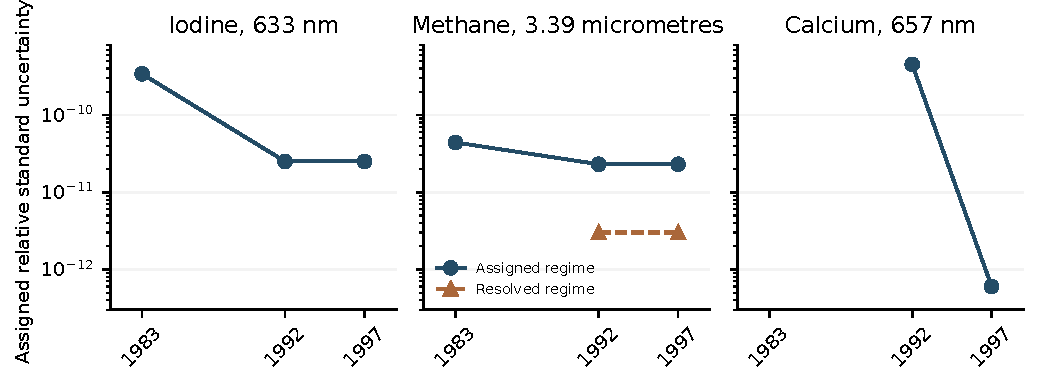
\includegraphics[width=\linewidth]{uncertainty_modes.pdf}
\caption{Selected assigned-uncertainty trajectories. *The 1983 points are explicitly stated relative standard deviations. Connecting lines identify documentary families, not controlled instrument histories. Methane is split into two regimes; calcium's large decrease accompanies changed realization conditions. Sources: the three CIPM lists.}\label{fig:modes}
\end{figure}

Classification can also change without withdrawal. The 576 nm iodine-stabilized dye or doubled He--Ne entry moves from the stabilized-laser section in 1992 to section 2.3, under spectral lamps and other sources, in 1997. Its assigned frequency, wavelength, and standard uncertainty are retained. A comparison confined to section 1 would incorrectly record disappearance. An audit of historical standards therefore requires identity, conditions, convention, and documentary location, not just a list of section headings or species.

\section{The Canadian laboratory: continuity as work}
\subsection{Modernization around an operating service}
The international lists establish what was authorized; they do not explain the local pace of replacement. The NRC's report of 8 August 2000 provides a more specific view. Its gauge-block interferometer had undergone repeated changes since its conception in the 1950s. The report dates the last major software upgrade to 1982 and a hardware upgrade to 1997. Further work proceeded in stages because extended interruption would disrupt routine calibration \citep[pp.~1--3]{decker2000}.

The report describes testing modules separately and then testing the combined system alongside the older software. The purpose was continuity of evaluated output across a change in implementation. It also describes replacing the cadmium lamp with laser sources better suited to image processing \citep[pp.~3, 5]{decker2000}. This gives a concrete local reason for replacement beyond a new definition or the smallest uncertainty in an international list. The source does not establish a single retirement date for all cadmium use at NRC, and no such date is inferred here.

The BIPM activity report exposes another aspect of persistence. In 1992 a faulty tube in a methane reference system obtained from VNIIFTRI was replaced during a visit by Yu.~S.~Domnin, and the system was checked. A different reference tube was replaced by one designed at BIPM. The report also explains that discharge tubes and methane cells were not commercially available, requiring in-house work to maintain the stabilized lasers \citep[pp.~163--164; French pp.~48--49]{cipm1992}. These details identify repair, particular components, and skilled collaboration as conditions of maintaining access to a nominally universal unit. They do not warrant a general claim about national dependency or the motives of the participants.

\subsection{A source-linked reconstruction of the uncertainty budget}
The NRC report supplies an especially useful quantitative check on the relation between a reference source and an industrial calibration result. Its Table 1 gives contributions to length uncertainty from fringe reading, wringing, phase change, geometry, laser drift and calibration, temperature, and the refractive index of air. These contributions already include sensitivity coefficients. Reconstructing the published quadrature calculation gives
\begin{equation}\label{eq:budget}
 u_{\mathrm{rows}}^2(L)=\sum_i a_i^2+L^2\sum_i b_i^2
 =153+0.018238L^2\quad\mathrm{nm}^2,
\end{equation}
where $L$ is in mm. This is arithmetic on displayed source entries, not a new measurement of the instrument. Higher-order contributions are retained as supplied in the report. The two laser terms contribute $(0.005L)^2+(0.001L)^2$.

The report separately prints a rounded summary $U=2\sqrt{12.4^2+0.144^2L^2}$ nm. Summing the displayed rows yields coefficients of approximately 12.369 and 0.135048, so it does not reproduce the summary exactly. We preserve both. The underlying unrounded calculation is unavailable, and some displayed entries, particularly $0.1L$ for alignment, are coarse. The difference should not be silently ``repaired'' or attributed to an error without further evidence. Table~\ref{tab:budget} shows its practical scale.

\begin{table}[htbp]\centering\small
\caption{Reconstruction from NRC 42753, Table 1. Expanded uncertainties use $k=2$. Variance shares and the last column use the displayed-row reconstruction.}\label{tab:budget}
\begin{tabular}{rrrrr}\toprule
Length & $U_{\mathrm{rows}}$ & $U_{\mathrm{summary}}$ & Laser variance & Remove-laser limit\\
(mm) & (nm) & (nm) & share (\%) & reduction (\%)\\\midrule
10 & 24.89 & 24.97 & 0.00168 & 0.00084\\
100 & 36.63 & 38.01 & 0.07752 & 0.03877\\
1000 & 271.23 & 289.07 & 0.14137 & 0.07071\\\bottomrule
\end{tabular}
\end{table}

At 1000 mm, laser drift and calibration together account for about 0.141\% of reconstructed variance. Optics and thermal terms dominate. Using the printed summary as the total instead gives about 0.124\% for the same two laser terms. Either treatment supports the limited conclusion that those terms are a small part of this reported budget. At shorter lengths, fixed end effects become more important (Figure~\ref{fig:budget}).

\begin{figure}[htbp]\centering
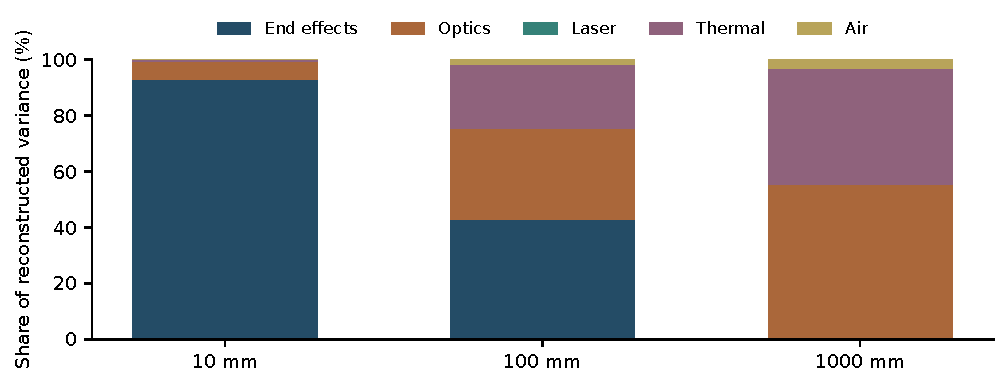
\includegraphics[width=\linewidth]{nrc_variance.pdf}
\caption{Variance shares reconstructed from the displayed NRC budget entries, grouped by physical role. The small laser share is included, although barely visible. These are contributions in a reported model, not variance components estimated from newly collected observations.}\label{fig:budget}
\end{figure}

A bounded counterfactual makes the interpretation explicit. If only the two laser terms were reduced to zero and every other displayed term remained fixed, the fractional decrease in standard uncertainty would be
\begin{equation}
 1-\sqrt{1-q_{\mathrm{laser}}(L)},\qquad
 q_{\mathrm{laser}}(L)=\frac{(0.005^2+0.001^2)L^2}{u_{\mathrm{rows}}^2(L)}.
\end{equation}
The resulting decrease at 1000 mm is about 0.071\%. This is a mathematical limit under a fixed-budget assumption, not an experiment, a causal prediction about an actual upgrade, or a claim that laser changes were useless. A different source could improve fringe analysis or other components as well. The calculation explains why improvement of a primary reference cannot simply be read as an equal improvement in a complete calibration service.

\section{Conditional authorization and the history of technical change}
The evidence supports three connected findings. First, a change in defining authority need not withdraw recognition from earlier sources. Krypton ceased to constitute the unit's definition but remained available through a specified route with an assigned uncertainty. The twelve legacy lamp wavelengths retained across the examined documents make that distinction numerically inspectable. The 1983 transition reorganized an existing plurality rather than replacing a homogeneous old system with a homogeneous new one.

Second, the later registers recognized different technical capacities without making them different metres. Their uncertainties were attached to regimes: cells, beams, trapped ions, correction procedures, and stabilization practices. The gains were uneven, and reporting conventions affected how large they appeared. What looked like a table of numbers also allocated conditions under which a source could be used with international authority. This allocation remained revisable while the definition stayed stable.

Third, local replacement had its own operational criteria. NRC's staged upgrades and BIPM's maintenance work show how service continuity and component availability mediated technical change. The Canadian record links source replacement to image-processing performance, while the budget reconstruction locates laser calibration inside a broader measurement system. These documents make the relationship between global authorization and local implementation concrete without requiring adoption rates or intentions that the sources do not supply.

The practical implication is for the design of historical and technical registers. A versioned record should preserve four things together: the legal or institutional status of the source, its identity and realization regime, the uncertainty convention, and the conditions governing its use. A table that retains only the latest numerical value cannot answer whether a source was withdrawn, relabeled, subdivided, or authorized under tighter conditions. The accompanying data and code implement this documentary discipline for a small corpus. They are an inspection aid, not a general certification system or a new metrological standard.

\section{Limits and conclusion}
This study concerns selected international documents and two institutional settings. It establishes documentary retention, changes in assigned uncertainty, and specific reported maintenance practices. It does not establish how many lamps remained in service, who could afford the competing routes, how national delegations negotiated particular wording, or how widely the recommendations were followed. Those questions require additional correspondence, procurement records, laboratory logs, and institutional comparisons. Official English translations and current web transcriptions also need to be distinguished from the authoritative French decisions and printed proceedings.

The arithmetic is descriptive and reconstructive. No sampling-based significance test is appropriate for a transcription of this bounded documentary corpus. Dependencies among recommended values prevent treating editions as independent experimental replications. In the Canadian case, displayed rounded entries and a separately printed summary do not fully agree, and both remain visible. These limits define what the findings mean rather than invalidating the exact comparisons they support.

The metre's redefinition in 1983 did more than replace the object named in a definition. It redistributed how existing sources acquired authority and how future improvements could be admitted. The older sources did not all disappear when one ceased to define the unit. Their afterlife was organized through conditional recommendations, maintained components, and staged changes to working services. Following these different timescales makes technical continuity visible as an institutional and material achievement.

\section*{Data and code}
The reproducibility package contains the source catalogue and retrieval hashes, 31 assigned-regime records, the independent 1963 and 1997 legacy-wavelength transcriptions, the 25-entry NRC uncertainty budget, analysis scripts, verification tests, and figure source code. All numerical tables and figures can be regenerated locally. The repository is available at \url{https://github.com/shi1720/metre-afterlife}. Source documents remain with their institutional providers; the package distinguishes transcribed data from original source files.

\appendix
\section{Audit trail and numerical interpretation}
The 1983 entries are in CIPM Recommendation 1, sections 1.1--1.5 and 2.1--2.2; their French printed list is at proceedings pp.~25--28. The 1992 list is at pp.~141--144 of the English proceedings; the unresolved methane unit is verified at p.~142. The BIPM maintenance narrative is in the same volume at pp.~163--164. The 1997 records retain their original numbered sections; the inherited lamp table is section 2.2 and the retained 576 nm laser is section 2.3. The 1963 table is at proceedings pp.~26--27. NRC 42753's budget is printed p.~7 (PDF p.~8 including the archive cover).

The implementation uses decimal arithmetic for $c/f$ and exact conversion of the legacy wavelength values. It uses ordinary floating-point arithmetic only for ratios and quadrature summaries, where displayed precision is far below numerical rounding error. Data files preserve printed precision and source conventions. Tests distinguish internal numerical consistency from equivalence of apparatus and from accuracy of the original experiment. The wavelength-pair check passes for 28 pairs; the twelve legacy conversions match exactly. The code also retains the location of the reclassified laser, so a section-based deletion cannot be mistaken for documentary withdrawal.

The standard-deviation comparisons in Table~\ref{tab:ratios} intentionally preserve the historical terminology. A fully uniform reassessment of the underlying measurement uncertainties would require the source measurements, weighting choices, correlations, and systematic-error assessments. That reassessment is outside the evidence reconstructed here. Consequently, ``13.6'' means the ratio of the two explicitly stated documentary quantities on the specified scale; it is not a newly estimated physical performance factor.

\begin{thebibliography}{99}
\bibitem[CGPM(1960)]{cgpm1960} CGPM. 1960. Resolution 6: Definition of the metre. 11th meeting. \href{https://doi.org/10.59161/CGPM1960RES6E}{doi:10.59161/CGPM1960RES6E}.
\bibitem[CIPM(1963)]{cipm1963} CIPM. 1963. Recommendation 1: \'Etalons secondaires de longueur d'onde. \emph{Proc\`es-verbaux}, 52nd session, pp.~26--27. \url{https://www.bipm.org/documents/20126/17315032/CIPM52.pdf}.
\bibitem[CGPM(1975)]{cgpm1975} CGPM. 1975. Resolution 2: Recommended value for the speed of light. 15th meeting. \href{https://doi.org/10.59161/CGPM1975RES2E}{doi:10.59161/CGPM1975RES2E}.
\bibitem[CGPM(1983)]{cgpm1983} CGPM. 1983. Resolution 1: Definition of the metre. 17th meeting. \href{https://doi.org/10.59161/CGPM1983RES1E}{doi:10.59161/CGPM1983RES1E}.
\bibitem[CIPM(1983)]{cipm1983} CIPM. 1983. Recommendation 1: Mise en pratique de la d\'efinition du m\`etre. \emph{Proc\`es-verbaux}, 72nd session, published 1984, pp.~25--28. \href{https://doi.org/10.59161/CIPM1983REC1E}{doi:10.59161/CIPM1983REC1E}.
\bibitem[Jennings et~al.(1987)]{jennings1987} Jennings, D.~A., R.~E.~Drullinger, K.~M.~Evenson, C.~R.~Pollock, and J.~S.~Wells. 1987. The continuity of the meter: The redefinition of the meter and the speed of visible light. \emph{Journal of Research of the National Bureau of Standards} 92(1):11--16. \url{https://nvlpubs.nist.gov/nistpubs/jres/092/jresv92n1p11_A1b.pdf}.
\bibitem[CIPM(1992)]{cipm1992} CIPM. 1992. Recommendation 3: Revision of the mise en pratique of the definition of the metre; and BIPM activity report. \emph{Proc\`es-verbaux}, 81st session, published 1993, pp.~141--144, 163--164. \href{https://doi.org/10.59161/CIPM1992REC3E}{doi:10.59161/CIPM1992REC3E}. Proceedings: \url{https://www.bipm.org/documents/20126/17315032/CIPM81.pdf}.
\bibitem[O'Connell(1993)]{oconnell1993} O'Connell, Joseph. 1993. Metrology: The creation of universality by the circulation of particulars. \emph{Social Studies of Science} 23(1):129--173. \href{https://doi.org/10.1177/030631293023001005}{doi:10.1177/030631293023001005}.
\bibitem[Quinn(1994)]{quinn1994} Quinn, T.~J. 1994. Mise en pratique of the definition of the metre (1992). \emph{Metrologia} 30:523--541. \href{https://doi.org/10.1088/0026-1394/30/5/011}{doi:10.1088/0026-1394/30/5/011}.
\bibitem[CIPM(1997)]{cipm1997} CIPM. 1997. Recommendation 1: Revision of the practical realization of the definition of the metre. 86th meeting. \href{https://doi.org/10.59161/CIPM1997REC1E}{doi:10.59161/CIPM1997REC1E}.
\bibitem[Decker and Pekelsky(1997)]{decker1997} Decker, Jennifer E., and James R.~Pekelsky. 1997. \emph{Uncertainty Evaluation for the Measurement of Gauge Blocks by Optical Interferometry}. NRC Document 41374. Institutional report version. \url{https://publications-cnrc.canada.ca/eng/view/ft/?id=0bc23e60-6f36-4398-9971-38da4af1f0e7}.
\bibitem[Quinn(1999)]{quinn1999} Quinn, T.~J. 1999. Practical realization of the definition of the metre (1997). \emph{Metrologia} 36:211--244. \href{https://doi.org/10.1088/0026-1394/36/3/7}{doi:10.1088/0026-1394/36/3/7}.
\bibitem[Decker et~al.(2000)]{decker2000} Decker, J.~E., K.~Bustraan, S.~de~Bonth, and J.~R.~Pekelsky. 2000. \emph{Updates to the NRC Gauge Block Interferometer}. NRC Document 42753, 8 August. \href{https://doi.org/10.4224/40003349}{doi:10.4224/40003349}.
\bibitem[Hall(2006)]{hall2006} Hall, John L. 2006. Nobel lecture: Defining and measuring optical frequencies. \emph{Reviews of Modern Physics} 78:1279--1295. \href{https://doi.org/10.1103/RevModPhys.78.1279}{doi:10.1103/RevModPhys.78.1279}.
\bibitem[Mitchell et~al.(2017)]{mitchell2017} Mitchell, Daniel Jon, Eran Tal, and Hasok Chang. 2017. The making of measurement: Editors' introduction. \emph{Studies in History and Philosophy of Science Part A} 65--66:1--7. \href{https://www.sciencedirect.com/science/article/abs/pii/S0039368117302339}{Publisher record}.
\bibitem[Sch\"odel et~al.(2021)]{schodel2021} Sch\"odel, Ren\'e, Andrew Yacoot, and Andrew Lewis. 2021. The new mise en pratique for the metre---a review of approaches for the practical realization of traceable length metrology from $10^{-11}$ m to $10^{13}$ m. \emph{Metrologia} 58:052002. \href{https://doi.org/10.1088/1681-7575/ac1456}{doi:10.1088/1681-7575/ac1456}.
\end{thebibliography}
\end{document}
